% !Mode:: "TeX:UTF-8"

\chapter{基于CD-Phone和CTC的语音识别}

无论是经典的HMM-GMM识别系统,还是基于HMM-DL的识别系统,均属于HMM的识别框架。
RNN的强大的时序序列建模能力在一定程度上可以学习HMM框架中的状态变化和跳转,
因此识别任务中RNN的引入,逐步淡化了HMM框架的作用。
HMM框架经过几十年的发展,已经非常的完善,
并且庞杂,深度学习引入识别任务后,
识别系统的结构进一步复杂,进行识别任务所需的步骤流程也越来越长。

因此,如何打破HMM框架,简化识别系统的流程,
进一步挖掘深度学习在语音识别任务上的能力成为目前语音识别研究的新热点之一\ucite{hannun2014deep, amodei2015deep, miao2015eesen}。
基于CD-Phone和CTC的语音识别是这些研究中的代表。
Phone和CD-Phone建模打破了经典的基于HMM状态CD-State建模的方法;
CTC的end-to-end的建模能力可以使基于深度学习的语音识别系统无需依赖经典的HMM-GMM框架,可以大幅度简化现有识别系统的流程。

本章分别介绍基于CD-Phone和CTC的语音识别,以及二者结合在声学建模中的应用。

\section{CD-Phone}

\subsection{传统建模单元CD-State} \label{seg:cdstate}

状态是HMM的基本建模单元,基于HMM的语音识别系统中每个音素Phone一般使用3状态的HMM。
在一般的语音识别系统中,音素的个数一般为几十个至上百个,例如TIMIT中音素数目为48,
汉语的语料库中即使带调的音素也不超过200。所以建模的单元数量少,建模不够精细。
为了对音素进行精确建模,可以进一步考虑音素所处的上下文,一般考虑音素所处位置的
前一个音素和后一个音素。例如对于音素b,我们可以建立a-b+c的三音素模型,其中a表示b
左边的音素,c表示b右边的音素。假设共有$N$个音素,考虑所有的上下文,一共可以得到$N^3$个三音素,
这样就解决了建模单元不够多,建模不够精细的问题。

然而,这样引进了新的问题。第一,建模单元太多,在训练数据固定的情况下,每个建模单元得到的训练数据不够充分;
第二,有一些三音素可能未在训练数据中出现,例如在汉语语料中,一般不会出现连续三个辅音的三音素,例如b-b+b,
z-z+z等。

\subsubsection{状态绑定Tied-State}

在经典的语音识别系统中,使用决策树和状态绑定(Tied-State)来解决这个问题。
状态绑定是指对于一个单音素的任意一个状态,该状态的一些三音素可以共享一个概率密度分布,即共享一个状态号,
例如a-b+a,e-b+a,i-b+a,o-b+a可以共享一个状态,因为他们的左上文\{a, e, i, o\}均为元音,
很可能在发音上具有相近性。通过状态绑定,一些发音相近的三音素状态可以共享相同的训练数据,
训练数据中未出现的三音素状态也可以绑定到已经出现的三音素上状态上,
这样即解决了训练数据稀疏和未出现三音素状态的建模问题。
最终,将决策树和状态绑定形成的三音素状态称为CD-State(Context Dependent State),以表明基本的聚类单元是状态,
并且状态是上下文相关的。

\begin{figure}
\centering
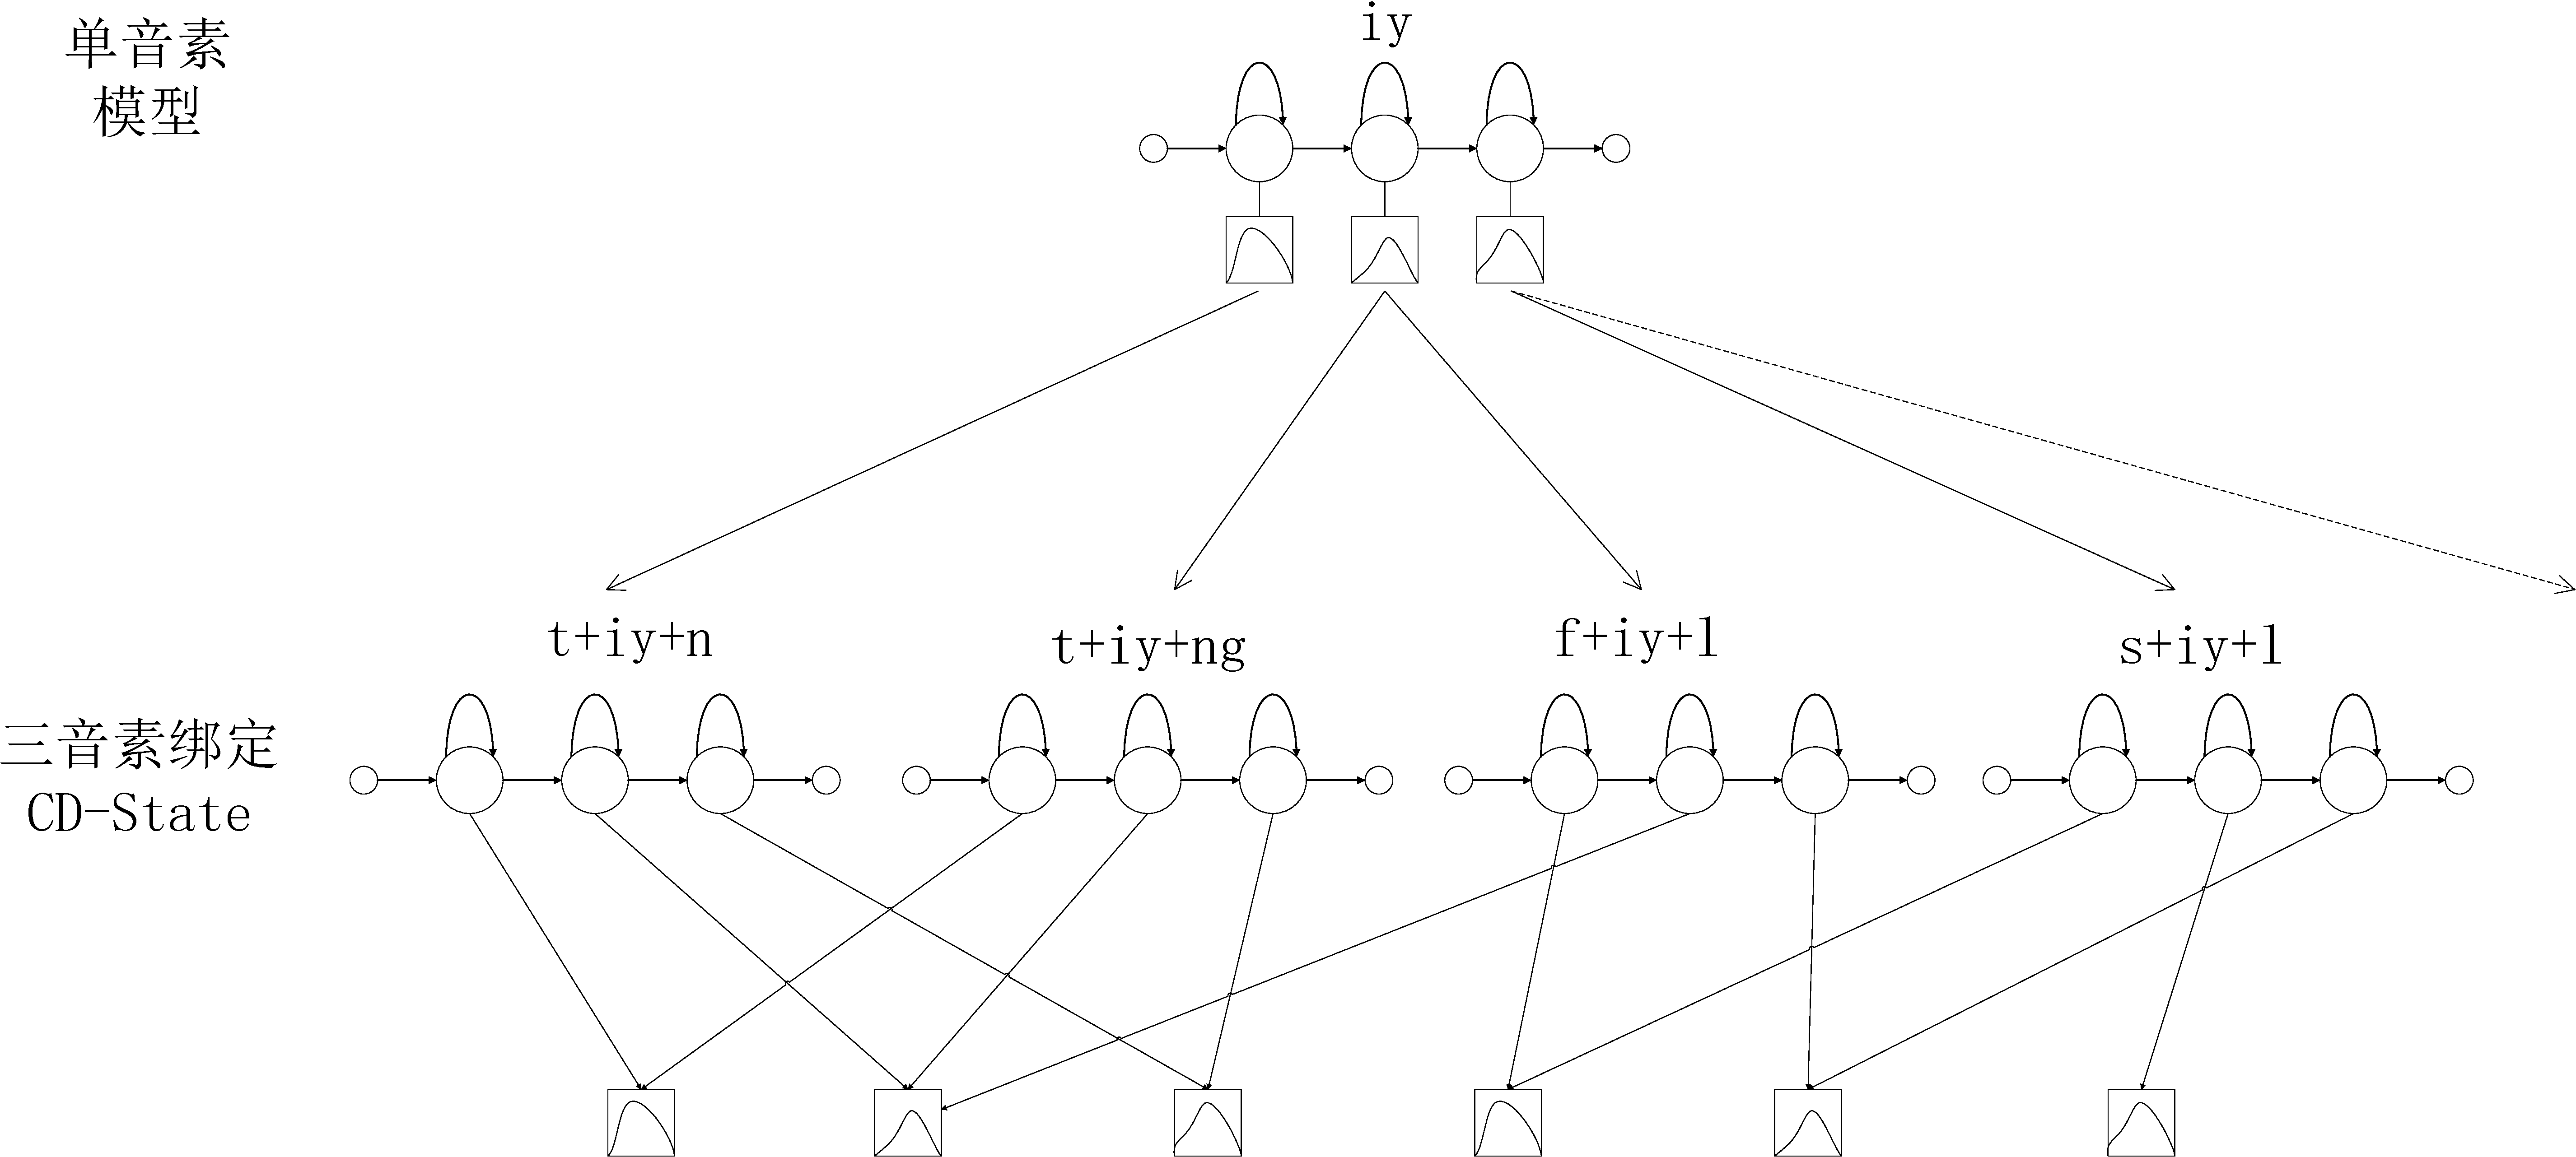
\includegraphics[width=1.0\textwidth]{figures/chapter4/cdstate-crop}
\caption{CD-State构建过程}
\label{fig:cdstate}
\end{figure}

HMM系统中CD-Stae的建立过程如图\ref{fig:cdstate}所示:
    \begin{enumerate}
        \item 首先建立和训练三状态的单音素的HMM模型。
        \item 使用已有单音素或三音素的模型得到三音素对齐,通过决策树建立状态绑定的三音素模型,迭代训练该模型。
        \item 重复2,直至模型训练充分。
    \end{enumerate}

\subsubsection{决策树}

上文提到建立CD-State的基本方法是决策树聚类。决策树是一个二叉树,在每个节点上都有相应的问题。
该问题相当于一个位置信息和一个音素集合,表示在当前层次,这个集合中的音素发音具有相近性。
对于三音素a-b+c,决策树会首先查看该节点的位置信息,通过位置信息确定是要判断b左边的音素还是右边的音素,
确定之后,然后判断该音素是否在该节点的音素集合中,若找到,
则走该节点的左子树,反之则走右子树。决策树的叶子节点表示最终三音素状态绑定的结果,
即该节点上的三音素共享相同的状态号。
对于任意一个三音素的给定HMM状态,通过该决策树就能查找到其最终的聚类结果。

\begin{figure}
\centering
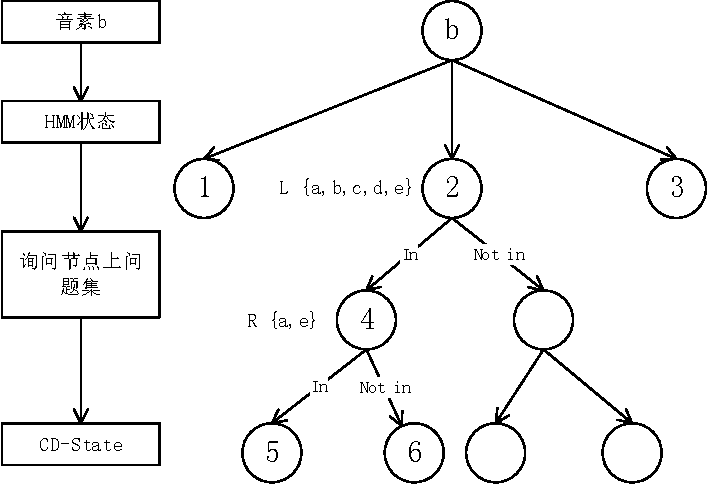
\includegraphics[width=0.6\textwidth]{figures/chapter4/tree-crop}
\caption{决策树示例}
\label{fig:tree}
\end{figure}

一个决策树的示例如图\ref{fig:tree}所示。根节点表示单音素,第二层表示单音素的三个状态,
第三层及其一下表示决策树状态决策过程。例如,对于三音素a-b+c的第二个状态,首先查找到状态2;
状态2上会看b的左边的音素是否在集合\{a, b, c, d, e\}中,判断为是,走到状态4;
接着判断a+b-c的右边状态是否在集合\{a, e\}中,判断为否,转到状态6;
状态6已经是叶子节点,查找结束。6即是三音素a-b+c的第二个HMM状态的聚类结果。

那么该决策树又是如何构建的呢?决策树是一个自上而下逐步构建的过程\ucite{young1994tree}。
首先,在单音素HMM状态的根节点上,所有的状态都被假设归位一类,然后计算其似然;
假设训练数据集为$S = ({x_1},...,{x_M}) \in ({R^N})$,其中$M$表示特征样本总数,$N$表示特征维度,
且各维特征相互独立(HMM-GMM系统中使用MFCC特征,使用对角高斯描述),则对于特征$\textbf{x}$,其似然为:
\begin{equation}
[P(x) = \frac{1}{{\prod\nolimits_{k = 1}^N {{{(2\pi \sigma _k^2)}^{1/2}}} }}\prod\limits_{k = 1}^N {\exp ( - \frac{1}{2}} \frac{{{{({x_k} - {\mu _k})}^2}}}{{\sigma _k^2}})
\end{equation}
对于集合$S$,其log似然为:
\begin{equation}
\begin{array}{l}
L(S) =  - \frac{1}{2}\sum\limits_{i = 1}^M {\left[ {\sum\limits_{k = 1}^N {\log (2\pi \sigma _k^2)}  + \sum\limits_{k = 1}^N {\frac{{{{({x_{ik}} - {\mu _k})}^2}}}{{\sigma _k^2}}} } \right]} \\
{\kern 1pt} {\kern 1pt} {\kern 1pt} {\kern 1pt} {\kern 1pt} {\kern 1pt} {\kern 1pt} {\kern 1pt} {\kern 1pt} {\kern 1pt} {\kern 1pt} {\kern 1pt} {\kern 1pt} {\kern 1pt} {\kern 1pt} {\kern 1pt} {\kern 1pt} {\kern 1pt} {\kern 1pt} {\kern 1pt} {\kern 1pt} {\kern 1pt} {\kern 1pt} {\kern 1pt} {\kern 1pt} {\kern 1pt}  =  - \frac{1}{2}\left[ {M\sum\limits_{k = 1}^N {\log (2\pi \sigma _k^2) + M} \sum\limits_{k = 1}^N {\frac{{\sigma _k^2}}{{\sigma _k^2}}} } \right]\\
{\kern 1pt} {\kern 1pt} {\kern 1pt} {\kern 1pt} {\kern 1pt} {\kern 1pt} {\kern 1pt} {\kern 1pt} {\kern 1pt} {\kern 1pt} {\kern 1pt} {\kern 1pt} {\kern 1pt} {\kern 1pt} {\kern 1pt} {\kern 1pt} {\kern 1pt} {\kern 1pt} {\kern 1pt} {\kern 1pt} {\kern 1pt} {\kern 1pt} {\kern 1pt} {\kern 1pt} {\kern 1pt}  =  - \frac{1}{2}\left[ {MN(1 + \log (2\pi ) + M\sum\limits_{k = 1}^N {\log (\sigma _k^2)} } \right]
\end{array}
\end{equation}
其中$\mu _k$表示集合$S$第$k$维的均值,$\sigma _k^2$表示集合$S$第$k$维的方差。
然后通过问题集中的一个问题将该节点分为两部分$S_l$和$S_r$,分别计算这两部分的似然和;
\begin{equation}
L({S_l}) + L({S_r}) =  - \frac{1}{2}\left[ {MN(1 + \log (2\pi ) + {M_l}\sum\limits_{k = 1}^N {\log (\sigma _{lk}^2) + {M_r}\sum\limits_{k = 1}^N {\log (\sigma _{rk}^2)} } } \right]
\end{equation}
遍历所有的问题集,选出似然增益和最大的问题作为最优问题;
\begin{equation}
\begin{array}{l}
{q^*} = \mathop {\arg \min }\limits_q L({S_{lq}}) + L({S_{rq}}) - L(S)\\
{\kern 1pt} {\kern 1pt} {\kern 1pt} {\kern 1pt} {\kern 1pt} {\kern 1pt} {\kern 1pt} {\kern 1pt} {\kern 1pt} {\kern 1pt} {\kern 1pt} {\kern 1pt} {\kern 1pt}  = \mathop {\arg \min }\limits_q \left[ {{M_l}\sum\limits_{k = 1}^N {\log (\sigma _{lk}^2) + {M_r}\sum\limits_{k = 1}^N {\log (\sigma _{rk}^2)} } } \right]
\end{array}
\end{equation}
其中$q^*$表示最优问题,并将根节点分为两部分。
然后递归的对所有分裂出来的新节点执行上述算法,
终止条件一般为,第一,每个节点上的在训练数据中的统计量已在小于设定临界值(避免该状态没有得到充分的训练数据);
第二,似然增益已小于设定阈值(该状态上所有绑定的三音素已足够相近); 两个条件满足其一即可。

\subsubsection{问题集}

在构建决策树时需要使用问题集,一个问题由一组声学上相近的音素组成,多个问题形成的集合即为问题集。
问题集的构建有两种方式:
\begin{enumerate}
\item 人工设计,根据语音和语言学的知识进行设计,与特定语言和任务相关,例如HTK\ucite{young2002htk}中即使用这种问题集。
\item 自动生成问题集,根据训练数据中的单音素对齐得到各个音素的发音特征,然后进行树聚类得到问题集。
\end{enumerate}
Kaldi\ucite{povey2011kaldi}中既可以使用人工设计的问题集,同时也能自动生成问题集,也可以两者结合使用。

\subsection{Phone和CD-Phone建模单元}

HMM建模的一个前提假设是状态的独立假设。在GMM和DNN中,当前时刻的状态预测仅与当前时刻的输出特征相关,
而在RNN中,因为RNN的内部状态,当前时刻预测输出不仅与当前时刻相关,而且还依赖历史时刻的输入。
所以,这一前提假设已经不成立,而且RNN强大的时序建模能力已经能够拟合HMM所描述的状态变化和跳转过程。
所以,直接使用Phone进行建模,使用RNN表述Phone的变化过程成为一种新思路。

使用Phone作为建模单元的过程如下:
\begin{enumerate}
\item 通过HMM-GMM系统得到状态对齐,进一步得到Phone对齐;
\item 直接Phone对齐训练基于Phone的RNN的声学模型。
\end{enumerate}
在解码时,HMM中的三状态约束使一个Phone至少持续三帧数据,基于Phone的解码时也要类似限制Phone的最小持续时间,
来保证解码出来的Phone的具有明确的时长持续变化,如图\ref{fig:duration}所示。

\begin{figure}
\centering
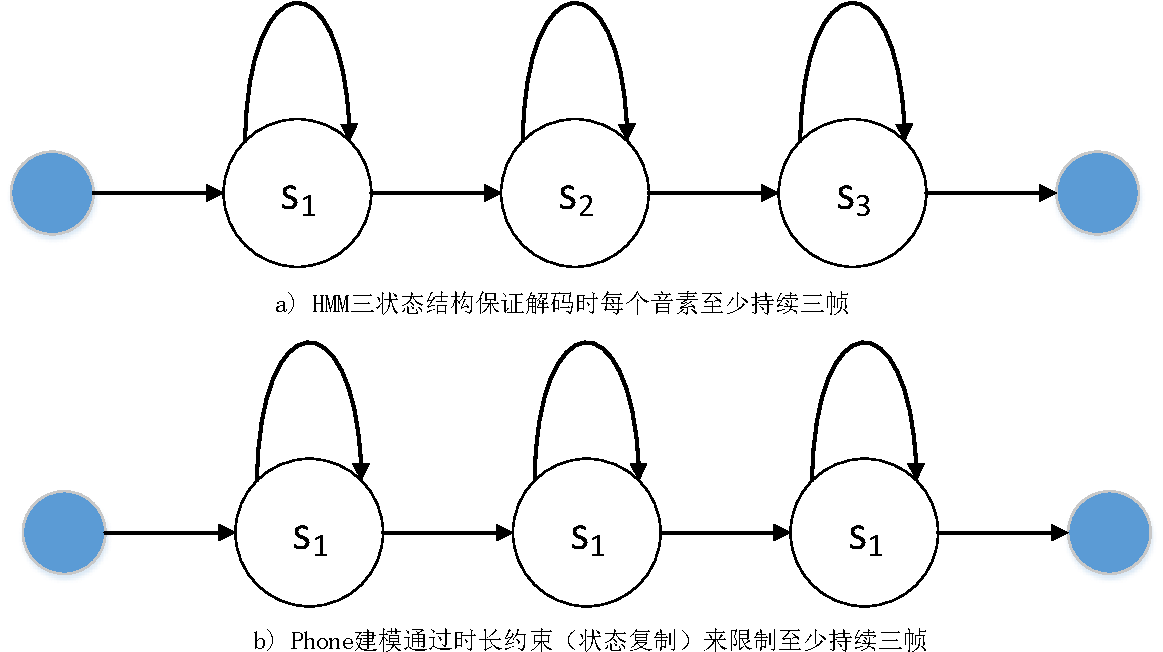
\includegraphics[width=0.6\textwidth]{figures/chapter4/duration-crop}
\caption{基于Phone的解码}
\label{fig:duration}
\end{figure}

但是,直接使用Mono Phone建模存在着与Mono Phone HMM状态建模相似的问题,即建模单元太少,建模不够精细。
使用与CD-State相似的概念,我们使用CD-Phone(Context Dependent Phone),给Phone加入上下文,
再通过聚类来结解决该问题。

CD-State聚类时,直接使用帧级状态对齐特征进行聚类。然而,Phone是一个有内部变化的建模单元,
在做聚类时需要考虑Phone的变化过程。Google在其CD-Phone\ucite{senior2015context}的工作中提出,
使用HMM-GMM系统中Phone的三个状态来描述Phone特征,使用三状态对齐的中值(均值)作为该Phone的特征,
如图\ref{fig:3middle}使用三状态的中值来表示Phone的聚类特征。

\begin{figure}
\centering
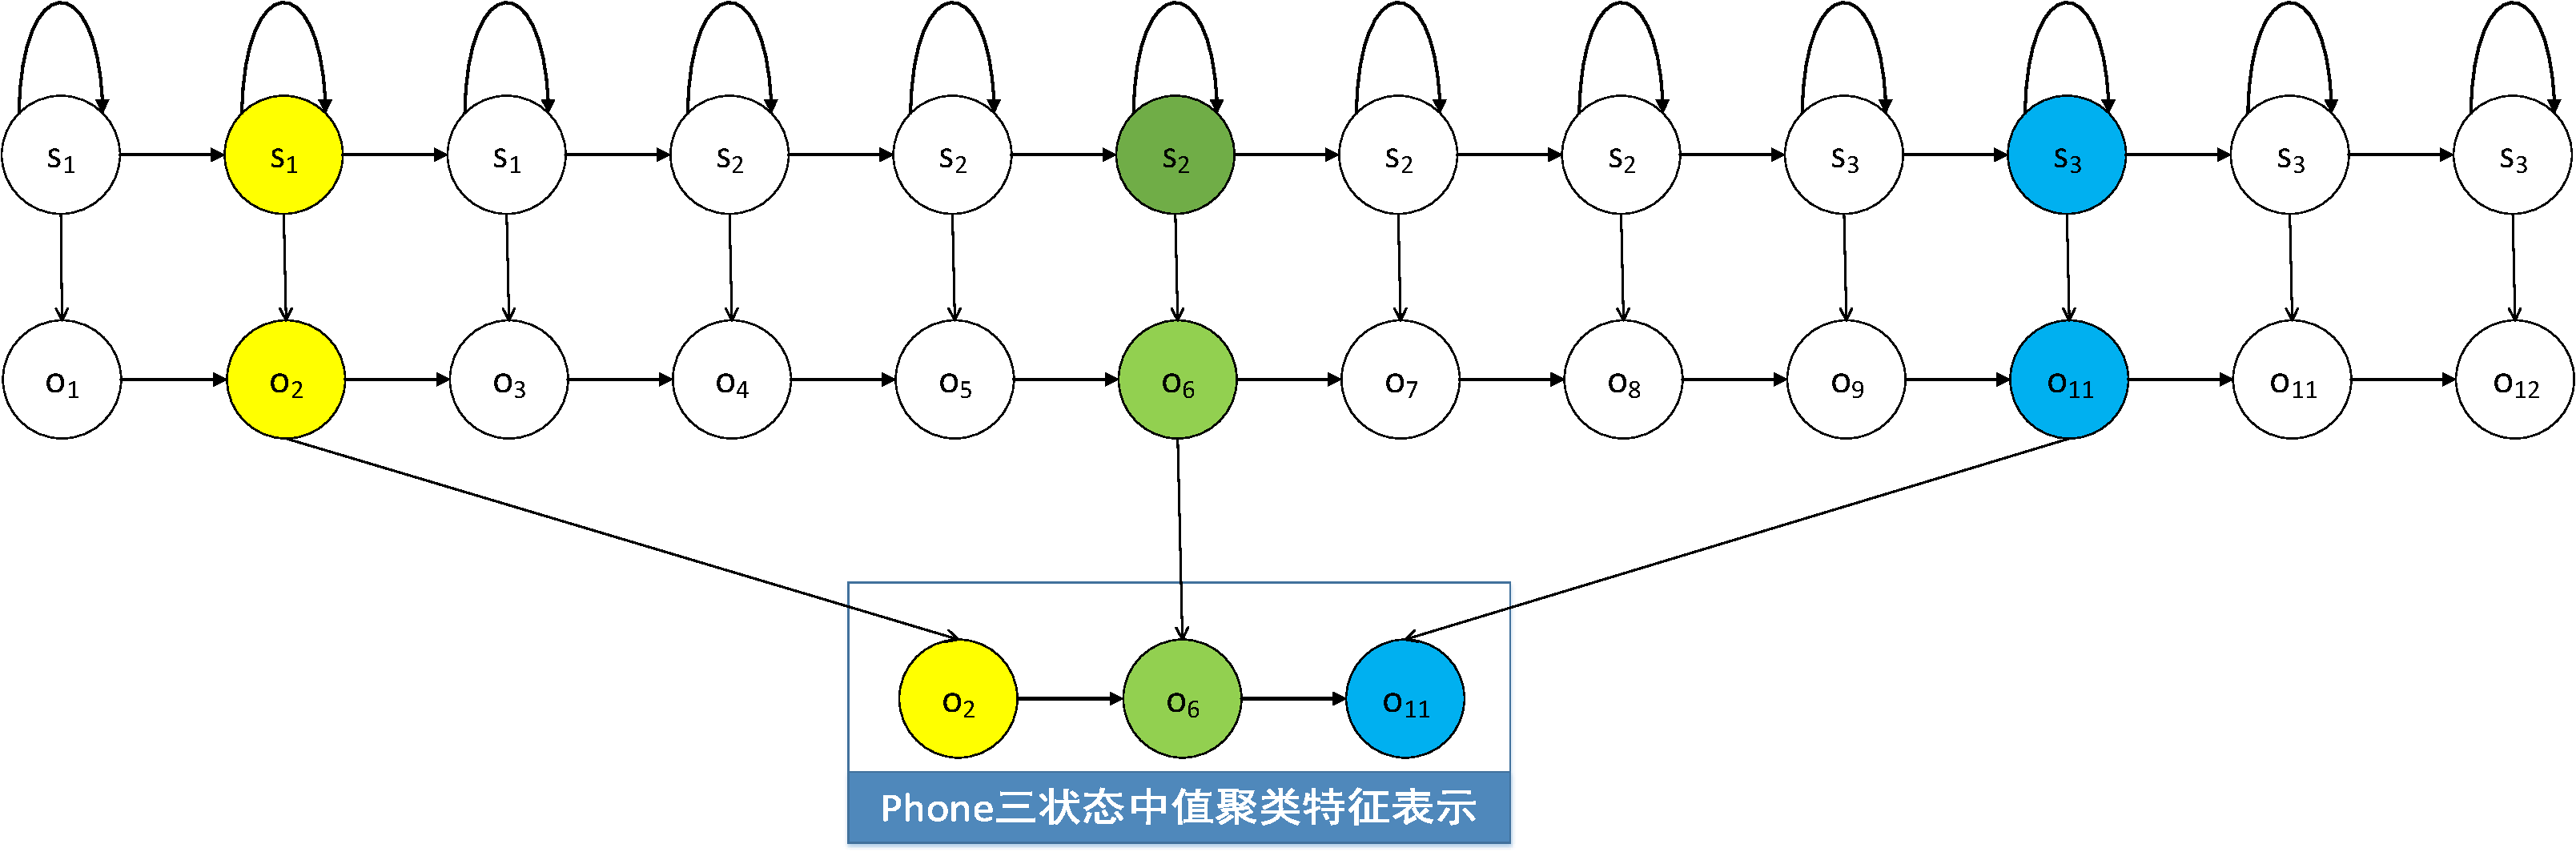
\includegraphics[width=0.8\textwidth]{figures/chapter4/3middle-crop}
\caption{CD-Phone聚类中Phone的特征表示}
\label{fig:3middle}
\end{figure}


使用CD-Phone作为建模单元的过程如下,
\begin{enumerate}
\item 通过HMM-GMM系统得到三音素状态CD-State对齐;
\item 按如上方法进行Phone特征统计,然后使用\ref{fig:cdstate}节类似方法使用问题集和决策树方法进行聚类;
\item 将CD-State对齐转换为CD-Phone的对齐;
\item 使用CD-Phone对齐训练基于RNN的CD-Phone的声学模型。
\end{enumerate}
在解码时,与Phone的解码类似,同样需要约束CD-Phone的最小持续时长。


\section{CTC}

如前文所述,基于深度神经网络的语音识别系统需要依赖HMM-GMM系统生成的状态对齐,复杂化了语音识别系统的流程。
语音识别本质上也是个序列标注任务,HMM方法是解决序列标注任务的一种经典方法之一。
CTC(Connectionist Temporal Classificatio)\ucite{graves2006connectionist, graves2012neural},
于2006年由Alex Graves提出,则是解决序列标注任务的另一种经典方法。

\subsection{基本概念}

在序列标注任务中,假设字符表的大小为$L$,CTC的softmax层输出则共有$L+1$个单元。
在给定输入的情况下,其中后$L$个用于预测当前时刻分别处在这$L$个字符上的概率;
另外一个为辅助单元,称之为blank(空白),用于预测在当前时刻不产生任何输出的概率,即空白。
所以,CTC在同一时刻的输出,可以使字母表中的任意一个字符,也可以是blank。

假设训练集为$S$,给定输入序列$\textbf{x}$,其长度为$T$,其对应字符标注序列记为$textbf{l}$,
$y_k^t$表示在$t$时刻观测到字符$k$的概率,其中$k<=L$; $k=0$表示输出blank单元的概率。
则序列$\textbf{x}$的任意一个等价序列$\pi$出现的概率可以表示为:
\begin{equation}
{\rm{p}}(\pi |\bf{x},S) = \prod\limits_{t = 1}^T {{\rm{y}}_{{\pi _t}}^t}
\end{equation}
其中$\pi  \in {L^{'T}}$,$L^{'T}$表示在输入序列$\textbf{x}$的标注中任意位置插入任意长度的blank,直至其总长度为$T$。
在后面介绍中,省略训练数据$S$,将$\rm{p}(\pi |\bf{x},S)$简记为$\rm{p}(\pi|\bf{x})$。

定义映射函数{\rm B},表示将CTC的预测序列经过消除连续出现的字符和去除blank之后的序列。
例如${\rm B}(a - ab - ) = {\rm B}( - aa -  - abb) = abb$。
直观上看,当从连续的字符到一个新字符,或者由blank到一个非blank字符时,即认为是新的字符。
我们称之为序列等价性。这个性质使CTC可以使用未分段的数据,因为该性质无需预先知道字符出现的时刻。
这里可以看出blank的另一个作用,即允许预测序列出现两个连续相同的字符,只要这两个字符之间存在blank即可。

根据序列等价性,$\bf{l}$的条件概率可以表示为:
\begin{equation}
p({\bf{l}}|{\bf{x}}) = \sum\limits_{\pi  \in {{\rm B}^{ - 1}}({\bf{l}})}^{} {p(\pi |{\bf{x}})}
\end{equation}

理论上,CTC可以使用任意结构的RNN,但为了对当前字符做更精准的预测,一般使用双向的RNN,
这样可以有效的利用前向和后向所有历史信息。

\subsection{前向后向算法}

在给出$p({\bf{l}}|{\bf{x}})$ 的形式之后,
我们可以使用与HMM的前向后向算法\ref{section:probability}类似的动态规划思想来计算$p({\bf{l}}|{\bf{x}})$的概率。
即该问题具有最优子结构,可以通过迭代填表的方式求得。

首先,定义${{\bf{l'}}}$表示在$\bf{l}$的开始,结束和相邻两个字符之间插入blank后的序列,则${{\bf{l'}}}$的长度为$2|{\bf{l}}| + 1$。
在计算过程中,我们允许从当前一个字符直接跳到下一个字符;或者从当前字符跳到自身;或者从当前字符跳到blank。

\subsection{目标函数}

\subsection{语音识别中的应用}






